%!TEX root = ./main.tex
\chapter{Studiul teoretic. Tehnologii folosite}\label{ch:2studiu_teoretic}
\textbf{TODO} O scurta introducere cu privire la ce reprezinta acest capitol

\textbf{TODO} Scrie in introducere si despre undele cerebrale!

Acest capitol are rolul de a prezenta aspectele fundamentale ale unei rețele neuronale și construirea rețelelor convoluționale din acestea. Pornind de la perceptron, element de bază, folosirea mai multor neuroni pentru a crea o rețea neuronală iar mai apoi, trecerea de la rețelele neuronale simple, la rețelele convoluționale.

\section{Rețele neuronale}
Rețelele neuronale artificiale reprezintă un sistem de calcul inspirat după modelul rețelelor neuronale biologice, atât ca și structură, cât și ca mod de procesare a informației. Neuronul artificial reprezintă unitatea elementară a unei rețele neuronale artificiale. Precum neuronul biologic, care conține dendrite și axioni, neuronul artificial imită această structură prin noduri de intrare si noduri de ieșire.
\subsection{Perceptronul}
Conceptele fundamentale ale neuronului artificial provin din modelul perceptronului introdus de către \textit{Frank Rosenblatt (1958)} \cite{rosenblatt1962principles} pe baza cercetărilor anterioare ale lui \textit{Warren McCulloch} și \textit{Walter Pitts} \cite{McCulloch:427611}.

Perceptronul primește o serie de valori la intrare, $x_1, x_2, x_3\dots$, și produce o singură ieșire. Pentru calculul ieșirii, sunt folosite așa numitele \textit{ponderi (weights)}, notate cu $w_1, w_2, w_3,\dots$, numere reale reprezentând importanța fiecărei intrări în determinarea ieșirii.
\begin{figure}[ht]
\center
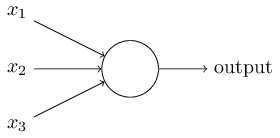
\includegraphics[width=7cm, keepaspectratio]{fig/cap2/perceptron.png}
\caption{Reprezentarea grafică a unui perceptron \cite{neuralnetbook:2015}}
\end{figure}

Astfel, ieșirea perceptronului, este determinată de suma ponderată $\sum_i x_iw_i$ comparată cu o valoare reală numită \textit{prag}. Această comparație reprezintă o funcție pentru determinarea ieșirii $y$, denumită \textit{funcție de activare}. Matematic, funcția de activare a perceptronului este reprezentată de o formă discretă a funcției \textit{treaptă unitate}, descrisă de ecuația \eqref{eq:perceptron-simplu}.
\begin{equation}
y = 
	\begin{dcases}
	0 & : \sum_i x_iw_i \le prag\\
	1 & : \sum_i x_iw_i > prag
	\end{dcases}
\label{eq:perceptron-simplu}
\end{equation}

Putem simplifica modul prin care perceptronii sunt descriși, rescriind $\sum\nolimits_i x_iw_i$ ca fiind produsul cartezian $x \cdot w$, unde $x$ și $w$ sunt vectori care conțin intrările $x_i$ respectiv ponderile $w_i$. A doua modificare pe care o putem face este să mutăm termenul $prag$ în partea stângă a inegalității, denumindu-l \textit{bias/offset}, $b=-prag$. Astfel, ecuația \eqref{eq:perceptron-simplu} devine:
\begin{equation}
y = 
	\begin{dcases}
	0 & : x \cdot w + b \le 0\\
	1 & : x \cdot w + b > 0
	\end{dcases}
\label{eq:perceptron}
\end{equation}

Bias-ul poate fii considerat ca o intrare suplimentară de valoate $x_0 = 1 \text{ și } w_0 = b$ care permite translatarea funcției de activare la stânga sau la dreapta.

\subsection{Perceptronul multistrat}
Prin conectarea mai multor perceptroni rezultă rețeaua numită „perceptronul multistrat” \textit{(Multi-layer Perceptron - MLP)}. Aceasta este formată în general de o succesiune de straturi de perceptroni complet conectați, compusă dintr-un strat de intrare, unul sau mai multe straturi ascunse \textit{(hidden layer)} și un strat de ieșire. Ieșirile unui strat reprezintă intrările pentru stratul următor. Rețeaua care conține mai multe straturi ascunse poartă denumirea de \textit{„rețea neuronală adâncă” ("deep neural network")}, iar în cazul în care aceasta conține un singur strat ascuns poartă denumirea de \textit{„rețea neuronală superficială” ("shallow neural network")}. \autoref{fig:mlp} prezintă o astfel de rețea. 
\begin{figure}[h]
\center
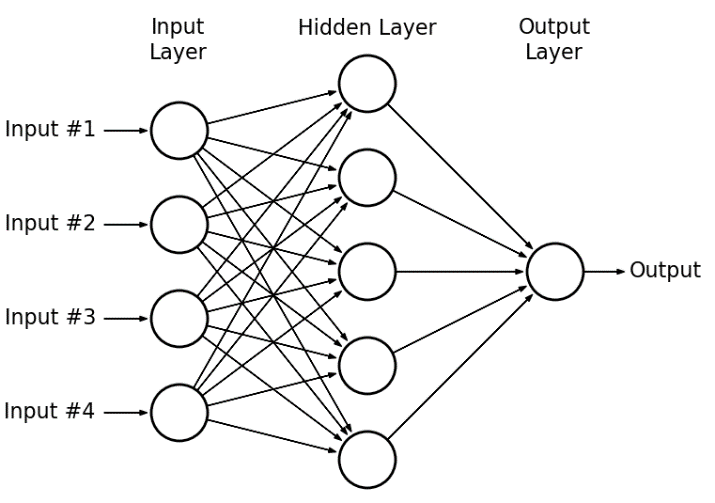
\includegraphics[width=10cm, keepaspectratio]{fig/cap2/mlp.png}
\caption{Rețea de tipul perceptron multistrat \cite{mlp-lakes}}
\label{fig:mlp}
\end{figure}

Rețeaua prezentată mai sus este de tip \textit{propagare înainte (feed-forward)}, adică, informația în rețea circulă într-o singură direcție, de la stânga la dreapta. Rezultatul procesării informațiilor de către primul strat de neuroni va reprezenta intrarea pentru stratul al doilea, astfel ieșirile acestuia având o semnificație mai abstractă și complexă comparativ cu primul strat. Cu fiecare strat ascuns adăugat rețelei, nivelul de abstractizare al informației va crește, astfel deciziile luate de rețea devenind tot mai sofisticate.

Limitarea acestui tip de rețea poate fii observată încercând să aplicăm schimbări mici ponderilor $w$ conexiunilor (sau a $bias$-ului) unui strat pentru a obține o schimbare mică a ieșirii rețelei. Analitic, acest lucru se rezumă la următoarea ecuație:
\begin{equation}
\Delta y\approx\sum_i\frac{\partial y}{\partial w_i}\Delta w_i + \frac{\partial y}{\partial b}\Delta b
\end{equation}
În realitate însă acest lucru nu se întâmplă întotdeauna. Aceste mici modificări pot determina schimbarea complet a stării\footnote{Acest lucru poate fi observat în graficul funcției de activare al perceptronului din \autoref{fig:sig+step+tanh+relu}}, spre exemplu de la 1 la 0. Acest comportament poate declanșa o schimbare foarte complicată și greu de controlat în întreaga rețea.

Limitarea dată de capacitatea perceptronului de clasificare binară, poate fii rezolvată însă folosind un alt tip de funcție de activare. 

\subsection{Neuronul}
Neuronul artificial este foarte asemănător cu perceptronul prezentat anterior. Acesta este format dintr-un vector de intrări $x$, un vector al ponderilor $w$, un bias $b$ și o ieșire $y$. Valorile vectorului de intrare $x$ nu sunt însă limitate la valorile 1 sau 0, neuronul sigmoid fiind capabil să proceseze valori reale. Precum $x$, ieșirea $y$ a neuronului poate lua valori reale. \autoref{fig:neuron} prezintă un astfel de neuron.
\begin{figure}[ht]
\centering
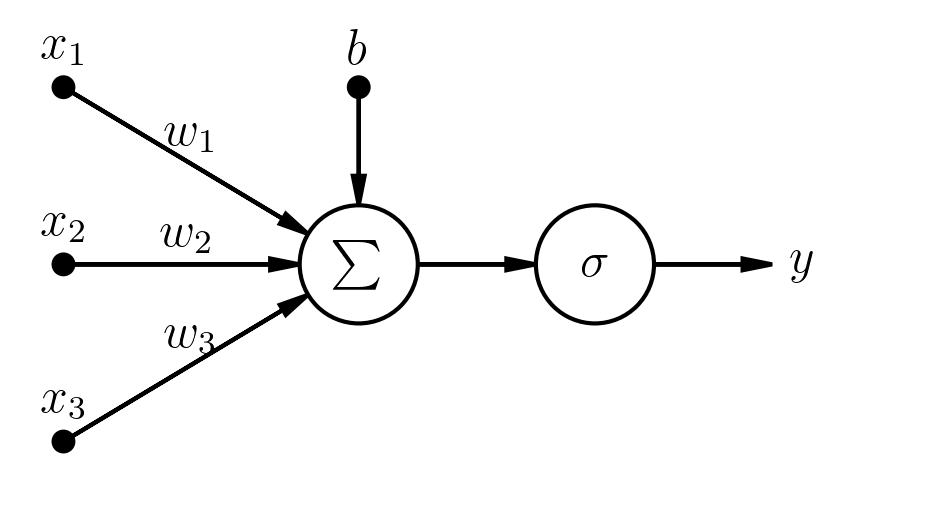
\includegraphics[width=10cm,keepaspectratio]{fig/cap2/artificial-neuron.png}
\caption{Reprezentarea grafică a unui neuron sigmoid}\label{fig:neuron}
\end{figure}

Neuronul care folosește \textit{funcția sigmoid} ca și funcție de activare, dată de ecuația \eqref{eq:sigm}, se numește neuron sigmoid și este cel mai simplu tip de neuron artificial datorită proprietăților funcției logistice la derivare\footnote{Derivabilitatea funcțiilor de activare este o cerință în cadrul folosirii algoritmului de antrenare prin back-propagation prezentat în \S\ref{subch:antrenare}}.

\begin{equation}
\sigma(z) = \frac{1}{1+e^{-z}} \quad,\text{unde }z= w\cdot x + b
\label{eq:sigm}
\end{equation}

Analizând graficele din \autoref{fig:sig+step+tanh+relu} putem observa faptul că funcția sigmoid este de fapt o versiune netezită a funcției treaptă unitate. Acest lucru ne asigură că schimbările mici efectuate atât în vectorul ponderilor $w$ cât și în $b$ vor fi reflectate în ieșire și că nu vom avea salturi bruște de la 0 la 1 la ieșirea neuronului.
Totuși, modelul perceptronului poate fii simulat folosind funcția sigmoid. Atunci când $z\rightarrow\infty$, $\sigma(z)\approx 1$, iar când $z\rightarrow-\infty$, $\sigma(z)\approx 0$. Folosind astfel de funcții de activare ne ajută să găsim ponderile potrivite mult mai ușor și putem afla felul în care modificările acestora afectează ieșirea.

În general, se folosesc funcții derivabile pe întreg domeniul de definiție, care nu au treceri bruște de la un capăt la altul, pentru a facilita antrenarea rețelei. În practică se mai folosesc funcții precum \textit{tangenta hiperbolică}:
\begin{equation}
\tanh(z)=\frac{e^z - e^{-z}}{e^z + e^{-z}}
\end{equation}
sau \textit{funcția unitate liniară rectificată (ReLU)}:
\begin{equation}
f(z)=\max(0,z)
\end{equation}

Mai jos sunt prezentate graficele diferitor funcții de activare.

\begin{figure}[h]
\centering
\subfloat[Funcția sigmoid]{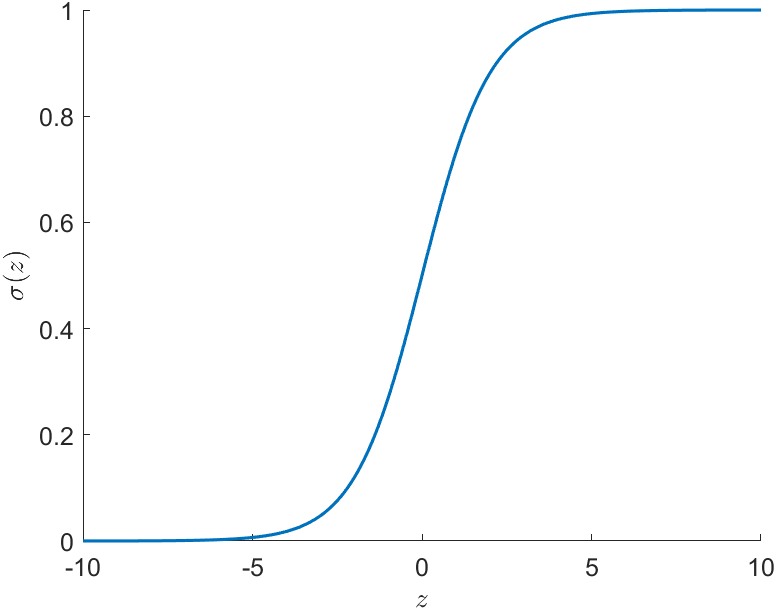
\includegraphics[width=6.8cm, keepaspectratio]{fig/cap2/sig.png}\label{fig:sigmoid}}
\qquad
\subfloat[Funcția treaptă unitate]{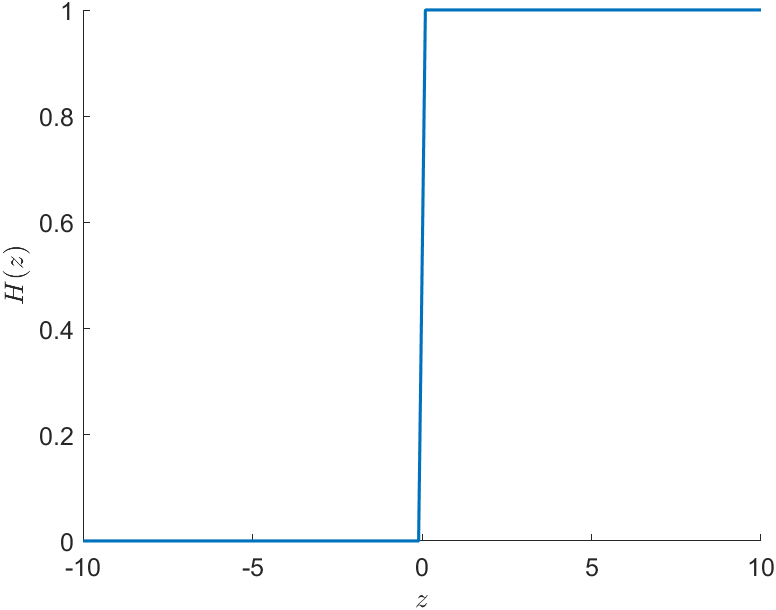
\includegraphics[width=6.8cm, keepaspectratio]{fig/cap2/step.png}\label{fig:step}}
\qquad
\subfloat[Funcția tangenta hiperbolică]{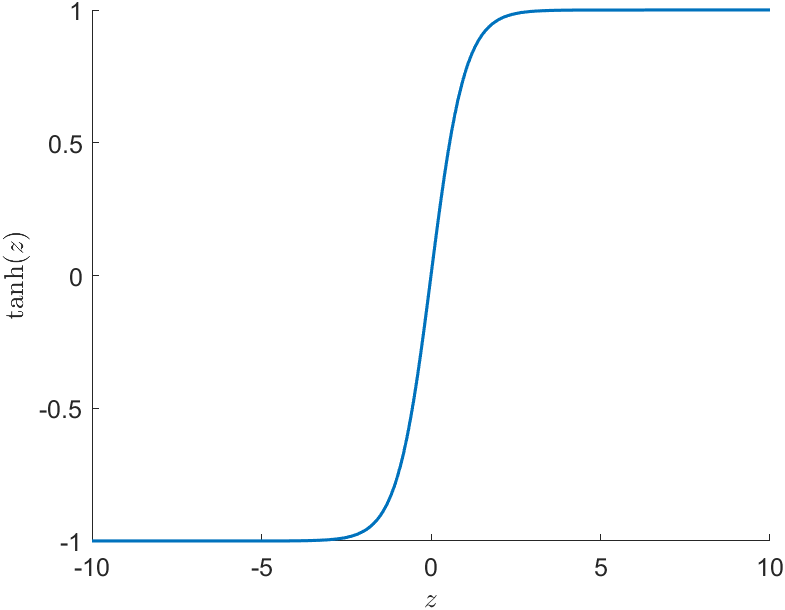
\includegraphics[width=6.8cm, keepaspectratio]{fig/cap2/tanh.png}\label{fig:tanh}}
\qquad
\subfloat[Funcția unitate liniară rectificată]{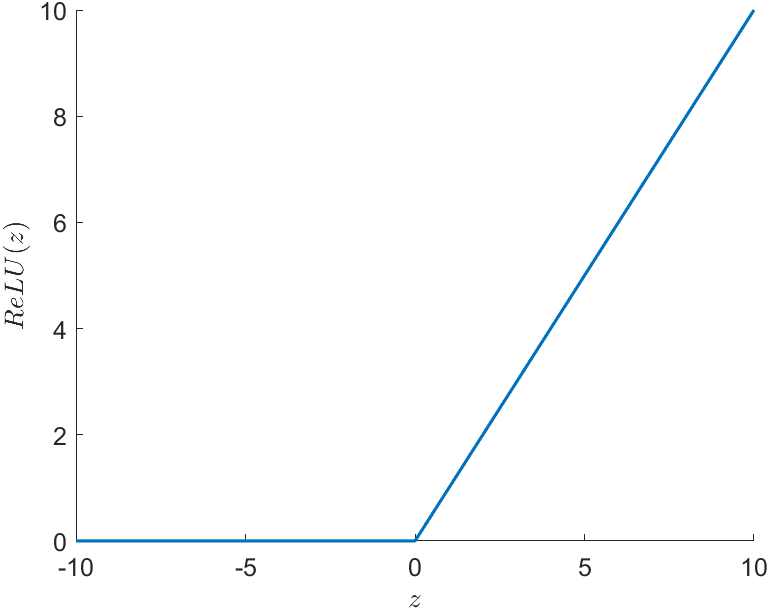
\includegraphics[width=6.8cm, keepaspectratio]{fig/cap2/relu.png}\label{fig:relu}}
\caption{Funcții de activare}\label{fig:sig+step+tanh+relu}
\end{figure}

Este necesar de menționat faptul că aceste funcții se folosesc în special pentru neuronii aflați în straturile ascunse ale rețelei, stratul de ieșire folosind de obicei funcții logistice pentru clasificări binare și funcția \textit{softmax} pentru clasificări multi-clasă.

\subsection{Antrenarea rețelelor}\label{subch:antrenare}
Algoritmul prin care se realizează antrenarea rețelelor de tipul feedforward, poartă denumirea de \textit{algoritm de propagare înapoi (back-propagation)}. Acest algoritm a fost făcut faimos de către David Rumelhart, Geoffrey Hinton, și Ronald Williams în 1986 \cite{Rumelhart1986}. Algoritmul constă în modificarea repetată a ponderilor conexiunilor din rețea în încercarea de a minimiza o funcție care reprezintă eroarea dintre rezultatul așteptat și cel obținut. Funcțiile folosite cu scopul de a fii minimizate se numesc \textit{funcții obiectiv} sau \textit{funcții de cost} (\S\ref{subch:f-cost}).

\subsubsection*{Ecuațiile algoritmului back-propagation}
Algoritmul clasic de back-propagation a fost inițial conceput să rezolve probleme de regresie folosind funcții de activare sigmoide. Totuși, acesta poate fii aplicat și problemelor de clasificare cu sau fară astfel de funcții de activare. Pentru a putea face o descriere matematică asupra modului de funcționare al algoritmului, este necesară folosirea următoarelor notații \cite{neuralnetbook:2015}:
\begin{enumerate}
\item $C$ pentru a reprezenta o funcție de cost
\item $w_{jk}^l$ pentru specificarea ponderii conexiunii de la neuronul $k$ în stratul $l-1$ către neuronul $j$ în stratul $l$.
\item $b_j^l$ pentru bias-ul neuronului $j$ din stratul $l$
\item $a_j^l$ pentru activarea neuronului $j$ din stratul $l$
\end{enumerate}
$a_j^l$ depinde de activarea neuronului din stratul $l-1$ conform ecuației
\begin{equation}
a_j^l=\sigma(\sum_k w_{jk}^l a_k^{l-1} + b_j^l)
\end{equation}
unde $k$ reprezintă toți neuronii din stratul $l-1$. Folosind aceste notații pot fii descrise cele patru ecuații fundamentale ale acestui algoritm:
\begin{enumerate}
\item Ecuația pentru determinarea erorii din stratul de ieșire $L$
\begin{equation}
\delta_j^L=\frac{\partial C}{\partial a_j^L}\sigma'(z_j^L)
\label{eq:out-err}
\end{equation}
\item Ecuație pentru determinarea erorii din stratul $l$ în raport cu eroarea din stratul $l+1$
\begin{equation}
\delta^l = ((w^{l+1})^T \delta^{l+1}) \odot \sigma'(z^l)
\label{eq:back-prop-err}
\end{equation}
\item Ecuație pentru determinarea ratei de schimbare a funcției de cost în funcție de orice bias din rețea
\begin{equation}
\frac{\partial C}{\partial b^l_j} = \delta^l_j
\label{eq:cost-w}
\end{equation}
\item Ecuație pentru determinarea ratei de schimbare a funcției de cost în funcție de orice pondere din rețea
\begin{equation}
\frac{\partial C}{\partial w^l_{jk}} = a^{l-1}_k \delta^l_j
\label{eq:cost-b}
\end{equation}
\end{enumerate}

\subsubsection*{Aplicarea algoritmului back-propagation}
Inițial toți parametrii rețelei (ponderile $w$ și bias-ul $b$) vor fii inițializați aleator\footnote{Nu este neapărat ca parametrii rețelei să fie inițializați aleator, existând mai multe metode de inițializare}. Urmează apoi etapa de propagarea înainte a datelor din setul de date de antrenare și a comparării rezultatului prezis în comparație cu cel real. Această eroare se calculează conform ecuației \eqref{eq:out-err}, iar mai apoi va fii propagată înapoi în rețea, strat cu strat, începând cu stratul $l = L-1$, conform ecuației \eqref{eq:back-prop-err}. Parametrii vor fi ajustați în funcție de gradientul funcției de cost conform ecuațiilor \eqref{eq:cost-w} și \eqref{eq:cost-b}. Gradientul funcției de cost se calculează folosind un algoritm de optimizare, cel mai folosit algoritm împreună cu back-propagation este metoda gradientului \textit{(gradient descent)}. Algoritmul se repetă pentru un numar stabilit de pași (aleși experimentali) sau până când eroarea $\delta^L$ scade sub o valoare impusă. Odată cu finalizarea algoritmului, rețeaua va fii pregătită să proceseze date pe care nu le-a întâlnit în setul folosit la antrenare și să facă predicții asupra acestora.
\begin{figure}
\centering
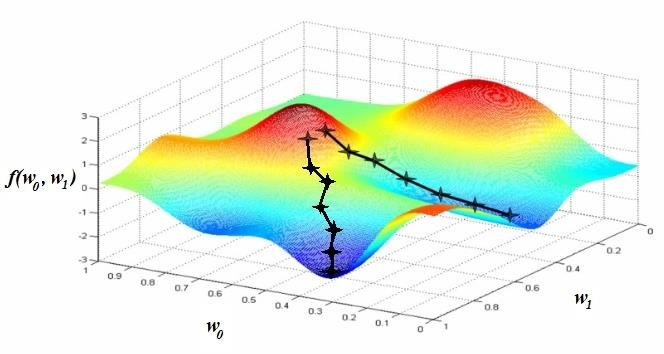
\includegraphics[width=10cm, keepaspectratio]{fig/cap2/grad-desc.jpg}
\caption{Ilustrarea algoritmului de optimizare gradient descent folosit în back-propagation\cite{vrejoiu:2019}}
\end{figure}

\subsection{Funcții de cost}\label{subch:f-cost}
O funcție de cost este o funcție de forma \cite{neuralnetbook:2015}
\begin{equation}
C(w,b,S^T,E^T)
\label{eq:cost-form}
\end{equation}
unde $w$ și $b$ reprezintă parametrii rețelei $S^T$ intrarea unui eșantion de date de antrenare și $E^T$ ieșirea dorită din eșantionul respectiv.

Rezultatul dat de asemenea funcții este un număr care reprezintă performanța rețelei de a face preziceri pe baza modificărilor aduse parametrilor acesteia. Se urmărește prin diferite \textit{tehnici de optimizare} minimizarea acestei funcții, valoarea returnată purtând denumirea de \textit{eroare/cost/loss}. În anumite situații însă, spre exemplu în cazul învățării cu întărire, scopul este de a maximiza această funcție, rezultatul fiind denumit \textit{recompensă}.

Atât funcțiile de cost, cât și tehnicile de optimizare ale acestora trebuie alese în funcție de problema în cauză, neexistând o soluție universal valabilă. Empiric, funcțiile de cost se pot împărți în două categorii:
\begin{itemize}
\item \textbf{pentru probleme de regresie}: eroarea medie absolută \textit{(L1 loss)}, eroarea medie pătratică \textit{(L2 loss)},  Huber Loss
\item \textbf{pentru problemele de clasificare}: funcția de cost logaritmică \textit{(cross-entropy)}, categorical cross-entropy, divergența Kullback–Leibler
\end{itemize}

\section{Rețele convoluționale}


\section{Undele cerebrale}
\textbf{TODO} Edit title